\section{Bosons, Bose-Einstein Condensation, and Helium-4}
\subsection{Housekeeping}
Reading assignment: Fermi liquid theory in Aschroft and Mermin p345-357. We don't have quite the mathematical tools to explain it, but the excerpt above gives a short qualitative introduction.

Midterm and Final: MT on First week of November. Both exams have the same structure; short in class portion (10-15 minutes), questions concerning things we are expected to know (e.g. $r_s = 2-6$ in metals, or temperature resistivity in Fermi liquid theory is $T^2$ etc.). Then there is a takehome portion with homework-level questions.

\subsection{Boson types and statistics}

But now we switch gears from fermions to bosons. There are two types of bosonic particles we consider in our discussion:
\begin{enumerate}[(a)]
    \item ``Real'' (number-conserving): $\phantom{i}^4\text{He}, \text{Rb}, \text{Na}, \text{K}, \ldots$
    \item ``Emergent'': Phonons (quanta of lattice vibrations), Magnons, \ldots 
\end{enumerate}
The main difference is that for the first class, the number of particles is conserved; the number of Helium atoms in a closed container is fixed. On the other hand, phonons can be created and destroyed out of thin air, so to speak. So there is no conservation law for them.

An important distinction between bosons and fermions is the type of statistics they obey. Mathematically, this is based on commutation relations; in terms of second quantization, bosons obey the commutation relations:
\begin{equation}
    \begin{split}
        &[a_\v{k}^\dag, a_\v{k'}] = \delta_{\v{k}\v{k}'}
        \\ &[a_\v{k}^\dag, a_\v{k'}^\dag] = [a_\v{k}, a_\v{k'}] = 0.
    \end{split}
\end{equation}
Recall the Pauli exclusion principle for fermions (which could be derived from the anticommutation relations); no such principle exists for bosons, of which any number are free to occupy the same quantum state. These commutation relations give rise to the BE distribution function:
\begin{align*}
    \bar{n}_\v{k} = \frac{1}{e^{\beta(\e_{\v{k}} - \mu)} - 1}
\end{align*}
where compared to the FD distribution, the sign in the denominator has flipped. 

\subsection{Deriving the Bose-Einstein Distribution}
Let's review how this distribution function comes about. Consider a non-interacting system:
\begin{equation}
    H = \sum_{\v{k}}(\e_{\v{k}} - \mu)a^\dag_{\v{k}}a_\v{k}
\end{equation}
The thermal average of any operator $\hat{O}$ is given by:
\begin{equation}
    \begin{split}
        \avg{\hat{O}}_\beta &= \frac{1}{Z}\sum_j \bra{j}\hat{O}\ket{j}e^{-\beta (E_j - \mu N)}
    \\  Z &= \sum_j e^{-\beta (E_j - \mu N)}.
    \end{split}
\end{equation}
where the matrix elements of $\hat{O}$ are weighted by the boltzmann factor, of which the partition function $Z$ is the sum of:
Note we use the grand canonic ensemble so we have the $\mu N$. We then have:
\begin{equation}
    \begin{split}
        \avg{\hat{n}_\v{k}} &= \frac{1}{Z}\sum_j \bra{j}a^\dag_{\v{k}}a_{\v{k}}e^{-\beta(\hat{H} - \mu\hat{N})}\ket{j}
        \\ &= \frac{1}{Z}\Tr(a_\v{k}^\dag a_\v{k} e^{-\beta(\hat{H} - \mu\hat{N})})
        \\ &= \frac{1}{Z}\Tr(a_\v{k} e^{-\beta(\hat{H} - \mu\hat{N})}a_\v{k}^\dag)
        \\ &= \frac{1}{Z}\Tr(a_\v{k} a_\v{k}^\dag e^{-\beta(\hat{H} - \mu\hat{N})}e^{-\beta(\e_{\v{k}} - \mu)})
        \\ &= \frac{1}{Z}\Tr((1 + a_\v{k}^\dag a_\v{k}) e^{-\beta(\hat{H} - \mu\hat{N})}e^{-\beta(\e_{\v{k}} - \mu)})
        \\ &= (1 + \avg{\hat{n}_\v{k}})e^{-\beta(\e_{\v{k}} - \mu)}
    \end{split}
\end{equation}
where in the first line, we take advantage of the fact that when $\hat{H}$ acts on its eigenstate, it gives back the eigenvalue. So we can pull the constant into the matrix element and convert the energy into the Hamiltonian. The second line we cast this expression as a trace. In the third line we use the cyclicity of the trace. In the fourth line we skip some math (but it can be done in detail) but this can be viewed as creating a single boson with energy $\e_{\v{k}}$. In the fifth line we use the bosonic commutation relations. In the sixth line we evaluate the expression. We can then solve for $\avg{\hat{n}_\v{k}}$ to obtain:
\begin{equation}
    \avg{\hat{n}_\v{k}} = \frac{1}{e^{\beta(\e_{\v{k}} - \mu)} - 1}.
\end{equation}
Note that a similar derivation can be done for Fermions to get the Fermi-Dirac distribution.

\subsection{Bose-Einstein Condensation}
BE Condensation occurs in real (or number conserving) bosons, most famously Helium-4 at low temperature. The easiest way to see this occurs is to consider the total number of bosons $N$:
\begin{equation}
    N = \sum_\v{k}\bar{n}_\v{k} = \sum_{\v{k}}  \frac{1}{e^{\beta(\e_{\v{k}} - \mu)} - 1}, \quad \e_{\v{k}} = \frac{\hbar^2\v{k}^2}{2m}
\end{equation}
Note that for real bosons $\mu \leq 0$; otherwise we would have $\bar{n}_{\v{k}} < 0$ for some $\v{k}$ which is forbidden. This implies that:
\begin{align*}
    e^{\beta(\e_{\v{k}} - \mu)} \geq e^{\beta\e_{\v{k}}}
\end{align*}
For this reason, we can bound the total number of bosons from above:
\begin{equation}
    \begin{split}
        N &\leq \sum_{\v{k}}\frac{1}{e^{\beta \e_{\v{k}}} - 1}
        \\ &= N_0 + \frac{\Omega}{(2\pi)^3}\int_0^\infty dk \frac{4\pi k^2}{e^{\beta\hbar^2k^2/2m} - 1}
    \end{split}
\end{equation}
where we have separated the sum into two terms; the $\v{k} = 0$ term (which is problematic as it formally diverges; it only comes about as we have discarded the chemical potential) and the rest of the sum rewritten as an integral, which we call $N'(T)$. $\Omega$ here is the volume. We leave the $N_0$ term for now and evaluate the $N'(T)$ by substitution. We let $x = \beta\frac{\hbar^2k^2}{2m}$ and $dx = \beta\frac{\hbar^2}{m}kdk$ so:
\begin{equation}
    N'(T) = \frac{\Omega}{(2\pi)^3}4\pi \sqrt{2}\left(\frac{m}{\beta\hbar^2}\right)^{3/2}\int_{0^+}^\infty \frac{\sqrt{x}dx}{e^x - 1} = C\Omega T^{3/2}
\end{equation}
The actual integral on the right is a finite constant (formally it can be evaluated by considering the Riemann zeta function), but we are really only interested in the temperature dependence, so we've lumped things into a constant $C$. It's also important that $N'(T)$ is extensive/grows proportionally to the system volume. Now we look at how BE condensation comes about from this. We rewrite the inequality as:
\begin{align*}
    N \leq N_0 + N'(T)
\end{align*}
We plot $N'(T)$ as a function of $T$. $N$ is fixed. There is some $T_c$ for which $N'(T)$ intersects $N$; above $T_C$, we have $N_0 = 0$, and below $T_c$ we have $N_0 > 0$. We have an extensive number of bosons in the $\v{k} = \v{0}$ state. This is what is known as BE condensation. In particular as we take $T \to 0$ all of the bosons occupy the ground state. This is not surprising; in the view of QM, if we try to minimize the energy of a set of bosons, we can just cram them all into the ground state (there is nothing preventing us from doing this; no Pauli exclusion)! However in terms of classical physics this phenomena was unusual.

\begin{figure}[htbp]
    \centering
    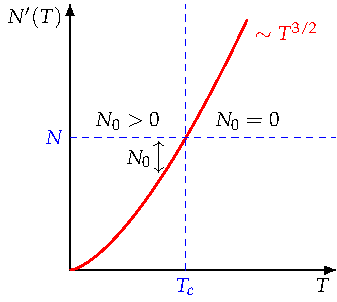
\includegraphics[]{Images/fig-superfluidN.pdf}
    \caption{Plot of the upper bound of excitated state bosons $N'(T)$ as a function of temperature $T$. Above some $T_c$, we have zero bosons in the ground state and so $N_0 = 0$. Below some $T_c$, we have that $N_0 > 0$ and so an extensive number of bosons occupy the $\v{k} = 0$ ground state; we therefore have Bose-Einstein condensation.}
    \label{fig-superfluidN}
\end{figure}

\subsection{Bogoliubov Theory of Helium-4}
This is a classic theory; 1946 (but still valid to this day)! Helium-4 was interesting from the early days of physics at it had interesting superfluid properties. Bogoliubov started off this explanation, and Landau later would give an argument for why Helium-4 is superfluidic (which we cover next lecture).

We consider weakly interacting (spinless) bosons described by the Hamiltonian:
\begin{equation}
    H = \sum_{\v{k}} \e_{\v{k}}a^{\dag}_{\v{k}}a_\v{k} + \frac{1}{2}\sum_{\v{k}\v{p}\v{q}}V_{\v{q}}a^\dag_{\v{k} - \v{q}}a^{\dag}_{\v{p} + \v{q}}a_\v{p}a_\v{k}
\end{equation}
where $V_\v{q}$ is a Fourier transform of a short-range interatomic potential; it is a short range interaction that dies off quickly outside of the Helium atom (on the order of an Angstrom). As usual, $\e_{\v{k}} = \frac{\hbar^2\v{k}^2}{2m}$. We assume (following Bogoliubov) that $V_{\v{q}}$ is weak and $T \ll T_c$. Then we expect the ground state to be close to a perfect BEC, where:
\begin{equation}
    \ket{\Phi^N_0} = (a^\dag_\v{0})^N\ket{0}
\end{equation}
Now we perform the following approximation:
\begin{equation}\label{eq-Napproxbogo}
    \begin{split}
        &a^\dag_\v{0}a_\v{0} \to \avg{a^\dag_\v{0}a_\v{0}} = N_0 \approx N
        \\&a^\dag_\v{0}a^\dag_\v{0} \to N_0
    \end{split}
\end{equation}
The first line: whenever we see the number operator, we take it to be its average value, which is large/close to the total number. The second line is less obvious, but consider $a_\v{0}^\dag a_{\v{0}}^\dag \ket{\Phi_0^N} = \sqrt{(N_0 + 1)(N_0 + 2)}\ket{\Phi_0^{N+2}}$ and we can then take $\sqrt{(N_0 + 1)(N_0 + 2)} \approx N_0$ for $N_0$ large. The assumption being made is that the Hamiltonian is always acting on a state close to the perfect BEC ground state, so we can approximate these operators as we have above. In the interaction term, we split all sums as:
\begin{align*}
    \sum_{\v{k}} = \sum_{\v{k} = 0} + \sum_{\v{k}}'
\end{align*}
and retain only terms containing at least only one power of $N_0$. This is a bit of a mess (as we have 8 sums to work with... ); we will not go through it explicitly, but we justify this approximation by saying that since $N_0$ is large, all terms without powers of $N_0$ are relatively small and hence can be neglected. The result is as follows:
\begin{equation}
    H \approx \sum_{\v{k}}\e_{\v{k}}a^\dag_\v{k}a_\v{k} + \frac{1}{2}N_0^2 V_0 + N_0V_0\sum_{\v{k}}' a_\v{k}^\dag a_\v{k} + N_0\sum_\v{q}'V_\v{q}a^\dag_{\v{q}}a_\v{q} + \frac{1}{2}N_0\sum_\v{q}' V_\v{q}(a_\v{q}a_{-\v{q}} + a_\v{q}^\dag a_{-\v{q}}^\dag)
\end{equation}
The first (kinetic energy) term remains unchanged. The second term comes from $\v{k} = v{q} = \v{p} = \v{0}$, The third term comes from $\v{p} = \v{q} = \v{0}$ or $\v{k} = \v{q} = \v{0}$ and so on. To simplify, we define:
\begin{equation}
    \begin{split}
        \eta_\v{k} &= N_0V_\v{k}
        \\ \hbar \Omega_\v{k} &= \e_\v{k} + \eta_\v{k}.
    \end{split}
\end{equation}
Notice also that $N_0 + \sum_\v{k}' a^\dag_\v{k}a_\v{k} \approx N$. where $N_0, N \gg N' = \sum_\v{k}' a^\dag_\v{k}a_\v{k}$. With this, let us combine some terms:
\begin{equation}
    \frac{1}{2}N^2V_0 = \frac{1}{2}V_0\left[N_0^2 + 2N_0\sum_\v{k}' a^\dag_\v{k}a_\v{k} + \ldots \right]
\end{equation}
Hence we can write the entire Hamiltonian as:
\begin{equation}\label{eq-He4aHamiltonian}
    H \approx \frac{1}{2}N^2 V_0 + \sum_{\v{k}}\left[\hbar \Omega_\v{k}a^\dag_\v{k}a_\v{k} + \frac{1}{2}\eta_\v{k}(a_\v{k}a_{-\v{k}} + a^\dag_\v{k}a^\dag_{-\v{k}})\right]
\end{equation}
We draw our attention to the last term(s); these are ``anomalous terms'', which \emph{do not} conserve particle number. This is a consequence of the Bogoliubov approximation. Physically, $a_\v{k}a_{-\v{k}}$ represent bosons $(\v{k}, -\v{k})$ ``disappearing'' into the condensate. The number of bosons in the condensate is so large that you do not have to keep track of the bosons in the condensate itself; we only need to keep track of the other particles as they disappear and appear out of it.

\subsection{Bogoliubov Transformations and Quasiparticle Spectrum}
Bogoliubov also developed a theory of how to treat such Hamiltonians. They can be diagonalized by means of Bogoliubov transformations:
\begin{equation}
    \begin{split}
        a_\v{k} &= \mu_\v{k}\alpha_\v{k} + \nu_\v{k}\alpha^\dag_{-\v{k}} \vert \alpha_\v{k} = \mu_{\v{k}}a_\v{k} - \nu_\v{k}a^\dag_{-\v{k}}
        \\ a_\v{k}^\dag &= \mu_\v{k}\alpha_\v{k}^\dag + \nu_\v{k}\alpha_{-\v{k}} \vert \alpha_\v{k}^\dag = \mu_{\v{k}}a^\dag_\v{k} - \nu_\v{k}a_{-\v{k}}
    \end{split}
\end{equation}
where we have the forwards transformations on the left and the inverse transformation on the right. Here, $\alpha_\v{k}$ are our new bosonic ``quasiparticle'' operators and $(\mu_\v{k}, \nu_\v{k})$ are real coefficients. We want this to be a canonical transformation, so we want these new $\alpha$ operators to satisfy the same commutation relations as the $a$s. This is important as it will place constraints on the $\mu_\v{k}$ and $\nu_{\v{k}}$. Let's see what happens:
\begin{equation}
    \begin{split}
        [\alpha_\v{k}, \alpha^\dag_{\v{k}'}] &= [\mu_{\v{k}}a_\v{k} - \nu_\v{k}a^\dag_{-\v{k}}, \mu_{\v{k}'}a^\dag_{\v{k}'} - \nu_{\v{k}'}a_{-\v{k}'}]
    \\ &= \mu_{\v{k}}\mu_{\v{k}'}[a_\v{k}, a^\dag_{\v{k}'}] + \nu_{\v{k}}\nu_{\v{k}'}[a^\dag_{-\v{k}}, a_{-\v{k}'}]
    \\ &= (\mu_{\v{k}}^2 - \nu_{\v{k}}^2)\delta_{\v{k}\v{k}'}
    \end{split}
\end{equation}
where we have used the known commutation relations for the $a$s. So we obtain the constraint:
\begin{equation}
    [\alpha_\v{k}, \alpha^\dag_{\v{k}'}] = \mu_{\v{k}}^2 - \nu_{\v{k}}^2 = 1.
\end{equation}

A comment: we want to find $(\mu_\v{k}, \nu_\v{k})$ such that the resulting $H$ is diagonal, that is:
\begin{equation}
    H = \sum_{\v{k}}\hbar \omega_\v{k}\alpha^\dag_{\v{k}}\alpha_\v{k} + E_0.
\end{equation}
So to this end we compute:
\begin{equation}
    \begin{split}
        \alpha^\dag_{\v{k}}\alpha_\v{k} &= (\mu_{\v{k}}a^\dag_\v{k} - \nu_\v{k}a_{-\v{k}})(\mu_{\v{k}}a_\v{k} - \nu_\v{k}a^\dag_{-\v{k}})
        \\ &= \mu_\v{k}^2a^\dag_\v{k}a_\v{k} + v_k^2a_{-\v{k}}a^\dag_{-\v{k}} - \mu_\v{k}\nu_{\v{k}}(a_\v{k}a_{-\v{k}} + a^\dag_{\v{k}}a^\dag_{-\v{k}})
    \end{split}
\end{equation}
Comparing this with the form of the Hamiltonian, we can see we are on the right track. The only terms to seem to not appear there are the $a_{-\v{k}}a^\dag_{-\v{k}}$s but we recognize the sum to run over all $\v{k}$ and so we can make a substitution there. We make an assumption that $\omega_\v{k} = \omega_{-\v{k}}$ and $\nu_{\v{k}}^2 = \nu_{-\v{k}}^2$ (we can check later that this is consistent) then:
\begin{equation}
    \sum_{\v{k}}\hbar \omega_{\v{k}}\alpha^\dag_{\v{k}}\alpha_{\v{k}} =  \sum_{\v{k}}\hbar \omega_{\v{k}}(\mu_{\v{k}}^2 + \nu_{\v{k}}^2)a^\dag_\v{k}a_\v{k} + \sum_{\v{k}}\hbar \omega_\v{k}\nu_{\v{k}}^2 - \sum_{\v{k}}\hbar \omega_{\v{k}}\mu_{\v{k}}\nu_{\v{k}}(a_\v{k}a_{-\v{k}} + a^\dag_{\v{k}}a^\dag_{-\v{k}})
\end{equation}
Comparison with the original Hamiltonian (Eq. \eqref{eq-He4aHamiltonian}) implies:
\begin{equation}
    \begin{split}
        \hbar \omega_\v{k}(\mu_{\v{k}}^2 + \nu_\v{k}^2) &= \hbar \Omega_{\v{k}}
    \\ 2\hbar \omega_{\v{k}}\mu_{\v{k}}\nu_{\v{k}} &= \eta_{\v{k}}
    \end{split}
\end{equation}
To solve for $\omega_{\v{k}}$ we square both equations and subtract:
\begin{align*}
    (\hbar \omega_{\v{k}})^2\left[(\mu_{\v{k}}^2 + \nu_{\v{k}}^2)^2 - 4\mu_{\v{k}}^2\nu_{\v{k}}^2\right] = (\hbar\Omega_{\v{k}})^2 - \eta_{\v{k}}^2
\end{align*}
but on the RHS We have $(\mu_{\v{k}} - \nu_{\v{k}})^2 = 1$ and so the dependence on $\mu/\nu$ drops out and we have:
\begin{equation}
    \hbar\omega_{\v{k}} = \sqrt{\hbar^2\Omega_{\v{k}}^2 - \eta_\v{k}^2} = \sqrt{\e_{\v{k}}(\eta_\v{k} + 2NV_\v{k})}
\end{equation}
which is one of the main results of Bogoliubov theory, the ``spectrum of quasiparticle excitations''. This spectrum will have interesting implications; among other things, it will be the basis for superfluidity in liquid He-4 according to the Landau argument. Let us discuss some special cases of this spectrum. 

\subsection{Quasiparticle Spectrum - Special Cases}
\subsubsection{Non-Interacting}
If the bosons are noninteracting, then $V_{\v{k}} = 0$ and so:
\begin{align*}
    \hbar\omega_{\v{k}} = \sqrt{\e_{\v{k}}^2} = \frac{\hbar^2\v{k}^2}{2m}
\end{align*}
so we indeed reproduce our prior result for free bosons.

\subsubsection{Contact Repulsion}
We take $V(\v{r}) = U\delta(\v{r})$ (i.e. the bosons repel when they are on top of each other). Since the FT of a dirac delta is just a constant, we have:
\begin{align*}
    V_{\v{k}} = \frac{U}{\Omega}
\end{align*}
for all $\v{k}$. We then have:
\begin{equation}
    \hbar\omega_\v{k} = \sqrt{\e_\v{k}(\e_\v{k} + 2(NU/\Omega))} = \begin{cases}
        \sqrt{\e_\v{k}E_0} \sim \abs{\v{k}}, \quad \e_{\v{k}} \ll E_0 \text{ (long wavelength = sound-like dispersion)}
        \\ \abs{\e_\v{k}} \sim \v{k}^2, \quad \e_{\v{k}} \gg E_0 \text{ (short wavelength = particle-like dispersion)}
    \end{cases}
\end{equation}
where we define $2(NU/\Omega) = E_0$. So the weak interactions of Helium modify the dispersion from particle like to sound-like at long wavelengths with linear dispersion relation.

\subsubsection{Typical Helium-4 Interaction}
The Fermi velocity for a typical interaction in Helium-4 scales with the wavevector as:
\begin{figure}[htbp]
    \centering
    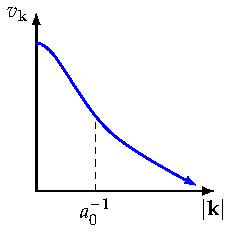
\includegraphics[]{Images/fig-Hevelocity.pdf}

    \caption{$v_\v{k}$ vs. $\abs{\v{k}}$ for a typical Helium-4 interaction.}
    \label{fig-Hevelocity}
\end{figure}

From this we obtain a dispersion relation that looks as follows:
\begin{figure}[htbp]
    \centering
    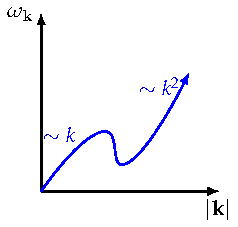
\includegraphics[]{Images/fig-Hedispersion.pdf}

    \caption{Dispersion relation for a typical Helium-4 interaction. The dispersion scales as $k$ for small $\abs{\v{k}}$ and as $k^2$ for large $\abs{\v{k}}$. The minima present in between the two regimes is known as the roton minimum.}
    \label{fig-Hedispersion}
\end{figure}

This concludes the Bogoliubov theory of Helium-4 in a nutshell. In the next assignment we will explicitly calculate the coefficients in the Bogoliubov transformation and other fun exercises.

\subsection{Landau Argument for Superfluidity}
To conclude, we cover Landau's argument for superfluidity for Liquid Helium 4. At the time, it was a known experimental fact that liquid Helium-4 would flow in a tube without friction. Experiments were also done where one would start spinning a bucket of Helium-4 at temperature above $T_c$, then the friction would cause it to rotate; then if one cooled the bucket down, the Helium would continue to rotate indefinitely.

Landau considered the following scenario. He considered a vessel of liquid Helium-4 and an object of large mass $M \gg m$ moving with velocity $\v{v}$. The question Landau asked was can the object relax its energy and momentum by emitting quasiparticle excitations? 

\begin{figure}[htbp]
    \centering
    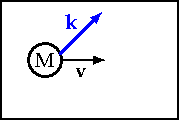
\includegraphics[]{Images/fig-Landaucartoon.pdf}
    \caption{Setting of the Landau argument for the superfluidity criterion. A heavy object with mass $M$ travels through a vessel of liquid Helium-4 with velocity $\v{v}$; can it relax its energy/momentum by emitting a quasiparticle of wavevector $\v{k}$?}
    \label{fig-Landaucartoon}
\end{figure}

We will show that it is impossible to conserve both energy and momentum and for the particle to relax so long as the object does not exceed a critical velocity $v_c$. Energy conservation and momentum conservation tell us that:
\begin{equation}
    \begin{split}
        \frac{1}{2}M\v{v}^2 &= \frac{1}{2}M\v{v}'^2 + \hbar \omega_{\v{k}}
        \\ M\v{v} &= M\v{v}' + \hbar\v{k}
    \end{split}
\end{equation}
These are the two equations we must satisfy if this process is allowed.
Squaring the second equation, we have:
\begin{align*}
    M^2\v{v}'^2 = M^2\v{v}^2 + \hbar^2\v{k}^2 - 2M\hbar \v{k} \cdot \v{v}
\end{align*}
We can divide out by $2M$ and combine the two conservation equations to find:
\begin{equation}
    \hbar \v{v} \cdot \v{k} = \frac{\hbar^2\v{k}^2}{2M} + \hbar \omega_\v{k}
\end{equation}
We consider $M \gg m$. and so we can neglect the $ \frac{\hbar^2\v{k}^2}{2m}$ term. Further we can let $\v{v} \cdot \v{k} = \abs{\v{v}}\abs{\v{k}}\cos\theta$ (where $\theta$ is the angle between the velocity and the wavevector of the emitted quasiparticle) and so:
\begin{equation}\label{eq-superfluidkomegak}
    \hbar \abs{\v{v}}\abs{\v{k}}\cos\theta = \hbar \omega_\v{k}
\end{equation}
For low enough velocities, the LHS will always be less than the RHS.

\begin{figure}[htbp]
    \centering
    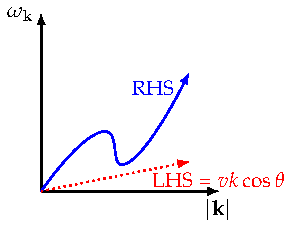
\includegraphics[]{Images/fig-graphicalsuperfluidsoln.pdf}

    \caption{Since $\cos\theta \leq 1$, for all $\theta$ the LHS ($\hbar vk\cos\theta$) of Eq. \eqref{eq-superfluidkomegak} will be less than the RHS ($\hbar \omega_\v{k}$).}
    \label{fig-graphicalsuperfluidsoln}
\end{figure}

The graphical solution shows that slow moving objects cannot dissipate energy and momentum in liquid Helium-4. We therefore have dissipationless motion, or superflow.

Note that one can solve for a critical velocity:

\begin{equation}
    v_c = \min_\v{k}\left(\frac{\omega_\v{k}}{\abs{\v{k}}}\right) \approx 1\si{cm.s^{-1}} \text{ in Helium-4}
\end{equation}

Note that the actual critical velocity is 10 times slower, due to neglected effects such as the creation of vortex rings etc. but nevertheless Landau's argument is an argument that provides some nice explanatory power!

Question: Why does argument not predict superfluid flow in general life situations? This is left as an exercise for the reader\dots

